  \documentclass[12pt]{article}

% Set up data, if you need to add a package, go here
\input{setup/packages.tex}


\begin{document}
\newcommand\numberthis{\addtocounter{equation}{1}\tag{\theequation}}
\newcommand\blankpage{%
    \null
    \thispagestyle{empty}%
    \newpage}

\thispagestyle{empty}
\setlength\headheight{0pt} 
\begin{center}

\begin{center}
\includegraphics[width=1\linewidth]{images/logo.jpg}            
\end{center}	

  \vspace{3 cm}

        {\Large\bfseries  ``Interaction-free measurements of different absorbers''\par}
        
        \vspace{0.5cm}
        {\Large\itshape by \\ \bfseries Gerardo José Suárez Rodríguez \par \par}
        

\vspace{2cm}

Submitted in Partial Fulfillment of the Requirements for the Degree \\
Master of Science, \\ Physics\\
Supervised by\par
Dr. Alonso Contreras Astorga  \\
Dra. Sara Guadalupe Cruz y Cruz\\


\vspace{1.5cm}
\large
\today

\end{center}

\clearpage
\restoregeometry
\justify
\tableofcontents
\addtocontents{toc}{\protect\thispagestyle{empty}}
\pagebreak
\pagenumbering{Roman}
\section*{Declaration}
I hereby certify that the material, which I now submit for assessment on the programmes of study leading to the award of Master of Science, is entirely my own work and has not been taken from the work of others except to the extent that such work has been cited and acknowledged within the text of my own work. No portion of the work contained in this thesis has been submitted in support of an application for another degree or qualification to this or any other institution.
\addcontentsline{toc}{section}{Declaration}

\vspace{2cm}
\begin{flushright}
-----------------------------------\\
Gerardo Suárez\\
\today
\end{flushright}
\pagebreak

%List of figures and tables, automatic from thesis.
\addcontentsline{toc}{section}{List of Figures}
\listoffigures\newpage
\addcontentsline{toc}{section}{List of Tables}
\listoftables\newpage
\blankpage{}
\section*{Acknowledgements}
Most figures were made using svgs from flaticom.com, the component library of Alexander Franzen and the noun project
\addcontentsline{toc}{section}{Acknowledgements}

\pagebreak



\blankpage{}

\section*{Abstract}
This is done at the end of the project
\addcontentsline{toc}{section}{Abstract}


\pagebreak


\blankpage{}

\section{Introduction}
\subsection{al final}
I am a subsection
\subsubsection{Sub Subsection Example}
I am a sub subsection
\pagebreak

\blankpage{}

\pagenumbering{arabic}

\section{Preliminars}

In this section, we will develop the necessary tools to understand the rest of this thesis. We will start with the process by which we will generate single photons which we will use as input for our Mach-Zehnder interferometer. We then develop the theory of a lossless beam splitter, then we use this to explore both the classical and quantum Mach-Zehnder interferometers. In the case of the quantum version, we explore different settings such as the Elitzur-Vaidman experiment and variations of it.

\subsection{Spontaneous parametric down conversion}

In this section, we will explore the quantum theory of spontaneous parametric down-conversion(SPDC), we will follow the approach taken in \cite{procopio} and \cite{multiphoton}. SPDC is a process where we make an intense laser beam go into a nonlinear crystal, occasionally one of the laser beam photons is annihilated and two photons of lower frequencies are created, Let us consider conservation of energy ($Energy_{l}=\hbar w_{l}$) where $w$ is the angular frequency, and conservation on linear momentum ($\mathbf{p_{l}}=\hbar \mathbf{k_{l}}$) :

\begin{equation}
w_{p}=w_{s}+w_{i} \qquad \mathbf{k_{p}}=\mathbf{k}_{s}+\mathbf{k_{i}},
\label{conservation}
\end{equation}

Where the sub-indices $p, i,s$ refer to pump, signal and idler respectively. This is the name often used in the literature for each of the photons in the process. Pump refers to the photons of the laser beam. Signal to the one we wish to use and idler to another one we'll use just to know the other one was indeed a single photon(using entanglement).

There are three types of SPDC, which are known as type-0, type-I, and type-II, respectively. The type of SPDC has to do with the polarization of each photon. In type-0 SPDC all photons have the same polarization.

In type-I, both produced photons have the same polarization which is orthogonal to that of the pump. In this kind of SPDC, both photons travel along the same light-cone.

In the last type of SPDC, type-II both produced photons that have orthogonal polarizations. In this type of SPDC, each photon travels along its light-cone. In this thesis, we are mainly concerned with the type-I SPDC process.

We will start our description of the SPDC process starting from the quantized electric field operator which can be written as:

\begin{align}
\textbf{E}(\textbf{r},t)&=\textbf{E}^{(+)} (\textbf{r},t) + \textbf{E}^{(-)} (\textbf{r},t),\\
\textbf{E}^{(+)} (\textbf{r},t)&=\frac{1}{\sqrt{V}} \sum_{\textbf{k},\nu} i(2 \pi \hbar w)^{\frac{1}{2}} \hat{a}_{\textbf{k},\nu} \hat{e}_{\textbf{k},\nu} e^{i(\textbf{k.r}-wt)}=[\textbf{E}^{(-)} (\textbf{r},t)]^{\dagger},
\end{align}

Where $V$ is the quantization volume, $\hat{e}_{\mathbf{k},\nu}$ is the unit polarization vector orthogonal to the wave vector, for two polarizations $\nu=1,2$, and $\hat{a}_{\textbf{k},\nu}$ is the  photon annihilation operator.the expression is summed over all possible modes of the field. The ladder operators, in this case, follow the commutation relation:

\begin{equation}
[\hat{a}_{\textbf{k},\nu},\hat{a^{\dagger}}_{\textbf{k},\nu}]=\delta_{\nu \nu'}\delta(\textbf{k}-\textbf{k'}).
\end{equation} 

The $\textbf{E}^{(+)} (\textbf{r},t)$ field operator acting on the vacuum state is:

\begin{equation}
\textbf{E}^{(+)} (\textbf{r},t)\ket{vacuum}=0,
\end{equation}

With the adjoint relation:

\begin{equation}
\bra{vacuum}\textbf{E}^{(-)} (\textbf{r},t)=0.
\end{equation}

Now, the Hamiltonian of an electromagnetic field can be written as:

\begin{equation}
H=\frac{1}{2}\int_{V} d^{3}r (\mathbf{D \cdot E}+\mathbf{H \cdot B}),
\end{equation}

where $\textbf{D}$ and $\textbf{H}$ which are the electric displacement and the magnetic field respectively are given in terms of the electric field ($\textbf{E}$) and the magnetic flux($\textbf{B}$) by the constitutive equations(with $\epsilon_{0} $ being the permittivity and $\mu_{0}$ the permeability of free space):


\begin{align}
\textbf{D}= \epsilon_{0} \textbf{E}+\textbf{P},\\
\textbf{H}=\frac{\textbf{B}}{\mu_{0}}-\textbf{M}.
\end{align}

We will neglect $\textbf{M}$ because we will assume that the laser beam is not strong enough to magnetize the crystal, so the Hamiltonian becomes:

\begin{equation}
H=\frac{1}{2}\int_{V} d^{3}r \left(\epsilon_{0}\mathbf{E \cdot E}+\mathbf{E \cdot P}+\frac{\mathbf{B \cdot B}}{\mu_{0}} \right)=H_{0}+H_{I}.
\end{equation}

The term $H_{I}$ has to do with the interaction of the laser pump and the crystal, it is the one we will be studying. We will consider the polarization to be nonlinear and the linear term to be included in $H_{0}$, the main contributor to the process is the second-order term in the nonlinear expansion (the expression for this second-order polarization $P_{i}^{(2)}$ can be found in \cite{boyd}):


\begin{align}
H_{I}&=\frac{1}{2} \int_{V} d^{3}r \textbf{E}.\textbf{P}^{(2)},\\
P_{i}^{(2)}&=\int_{0}^{\infty}dt_{1}\int_{0}^{\infty}dt_{2} \chi_{ijk}^{(2')}(t-t_{1},t-t_{2}) E_{j}(\textbf{r},t_{1}) E_{k}(\textbf{r},t_{2}),
\end{align}

where $\chi_{ijk}^{(2')}$ is the second-order nonlinear susceptibility, by substituting (12) in (11) and separating the fields in the creation and annihilation fields this can be written as:

\begin{align*}
H_{I}=\frac{1}{2} \int_{V}\int_{0}^{\infty}dt_{1}\int_{0}^{\infty}dt_{2} \chi_{ijk}^{(2')}(E_{i}^{(+)}E_{j}^{(+)}E_{k}^{(+)}+E_{i}^{(-)}E_{j}^{(+)}E_{k}^{(+)}+E_{i}^{(-)}E_{j}^{(-)}E_{k}^{(+)}+\\
E_{i}^{(+)}E_{j}^{(-)}E_{k}^{(+)}+E_{i}^{(+)}E_{j}^{(+)}E_{k}^{(-)}+E_{i}^{(-)}E_{j}^{(+)}E_{k}^{(-)}+E_{i}^{(-)}E_{j}^{(-)}E_{k}^{(-)}+E_{i}^{(+)}E_{j}^{(-)}E_{k}^{(-)}). \numberthis
\end{align*}

SPDC, as we mentioned before, is the annihilation of one photon and the creation of two. The only term compatible with this is $E_{i}^{(+)}E_{j}^{(-)}E_{k}^{(-)}$ as can be seen from equation (3), and its conjugate which means the reverse process. The other terms would not conserve energy  so we do not consider them:

\begin{equation}
H_{I}=\int_{V} d^{3}r \chi_{ijk}^{(2)} (E_{i}^{(+)}E_{j}^{(-)}E_{k}^{(-)}+H.C.),
\end{equation}

where  $H.C$ means hermitian conjugate and we redefined:

\begin{equation}
\chi_{ijk}^{(2)}(w_{1},w_{2})=\frac{1}{2}\int_{0}^{\infty}dt_{1}\int_{0}^{\infty}dt_{2} \chi_{ijk}(t_{1},t_{2})^{(2')}.
\end{equation}

Replacing the expressions for the fields, and approximating the sum to an integral we take $\sum_{\textbf{k}}\xrightarrow{}\int d^{3}k$:

\begin{align*}
&H_{I}=\int d^{3}k_{p}\int d^{3}k_{s}\int d^{3}k_{i} \sum_{\nu_{p},\nu_{s},\nu_{i}}\chi_{ijk}^{(2)}(w_{p},w_{s},w_{i}) (\hat{e}_{k_{p},\nu_{p}})_{i} (\hat{e}_{k_{s},\nu_{s}})^{\star}_{j} (\hat{e}_{k_{i},\nu_{i}})^{\star}_{k} \hat{a}_{\nu_{p}}(\mathbf{k_{p}})\hat{a^{\dagger}}_{\nu_{s}}(\mathbf{k_{s}})\\
&\hat {a^{\dagger}}_{\nu_{i}}(\mathbf{k_{i}})e^{i(w_{s}+w_{i}-w_{p})t} \int_{V}d^{3}r e^{i \Delta\textbf{k}.\textbf{r}}+H.C ,
\end{align*}

where we defined:
\begin{align}
\Delta \textbf{k}&= \mathbf{k_{p}}-\mathbf{k_{s}}-\mathbf{k_{i}},\\
\chi_{ijk}^{(2)}(w_{p},w_{s},w_{i})&=\frac{-iV}{(2\pi)^9}(2 \pi)^{\frac{3}{2}} (w_{p}w_{s}w_{i})^{\frac{1}{2}}\chi_{ijk}^{(2)}.
\end{align}

Since polarizations are fixed in SPDC, we actually do not sum over $\nu$ but have a single value for it. Also we will consider $\chi_{ijk}^{(2)}$ to vary so slowly(in k and r) that we can treat it as a constant over the integrals. We will define $\chi=\chi_{ijk}^{(2)} (\hat{e}_{k_{p},\nu_{p}})_{i} (\hat{e}_{k_{s},\nu_{s}})^{\star}_{j} (\hat{e}_{k_{i},\nu_{i}})^{\star}_{k}$ so we can write:

\begin{equation}
H_{I}=\chi \int d^{3}k_{p}\int d^{3}k_{s}\int d^{3}k_{i}\int_{V} d^{3}r \hat{a}_{\nu_{p}}(\mathbf{k_{p}})\hat{a^{\dagger}}_{\nu_{s}}(\mathbf{k_{s}})\hat {a^{\dagger}}_{\nu_{i}}(\mathbf{k_{i}})e^{i(w_{s}+w_{i}-w_{p})t}e^{i \Delta\textbf{k}.\textbf{r}}+H.C.
\end{equation}


Let us remember what the evolution operator definition is, let us use this to derive the Dyson series. Note that we will be using the $H_{I}$ because we will be working in the interaction picture (since $H_{0}$ is proportional to the number operator it only adds a global phase to the evolution of the system, the interaction Hamiltonian is $H_{I}$):


\begin{align}
U(t,t_{0})&=e^{\frac{1}{i \hbar} \int_{t_{0}}^{t} H_{I}(\tau) d\tau},\\
\ket{\psi(t)}&=U(t,t_{0})\ket{\psi(t_{0})},\\
i \hbar \frac{d}{dt}\ket{\psi(t)}&=H_{I}\ket{\psi(t)},\\
i \hbar \frac{d}{dt}(U(t,t_{0})\ket{\psi(t_{0})})&=H_{I}(U(t,t_{0})\ket{\psi(t_{0})}). 
\end{align}

By applying the Leibniz rule and because the equation must be valid for any ket, one can arrive to:

\begin{align}
i \hbar \frac{d}{dt}U(t,t_{0})=H_{I}U(t,t_{0}).
\end{align}

By direct integration, this can be written as an iterative integral equation, which is commonly known as Dyson series($U(t_{0},t_{0})=1$):

\begin{equation}
U(t)=1-\frac{i}{\hbar} \int_{t_{0}}^{t} H_{I} (\tau) d\tau.
\end{equation}

The laser beam or pump is in a coherent state \cite{leonhardt}:

\begin{equation}
\ket{\alpha}=e^{\frac{-|\alpha|^{2}}{2}} \sum_{n=0}^{\infty} \frac{\alpha^{n}}{\sqrt{n!}} \ket{n}.
\end{equation}

Coherent states are eigenstates of the annihilation operator with eigenvalue $\alpha$ which can be complex, it is known as the complex wave amplitude, this kind of state has the following properties:

\begin{align}
\langle H \rangle = \hbar w (|\alpha|^{2}+\frac{1}{2}),\qquad P_{n}=e^{-\langle n\rangle}\frac{\langle n \rangle^{n}}{n!},
\end{align}

where $P_{n}$ is the probability of finding n photons, it obeys poissonian statistics, our initial state is having the laser beam and no signal o idler photons that is a state $\ket{\alpha_{p},0_{s},0_{i}}$. Let us analyze the second order term of the Dyson series  $U_{1}=\frac{-i}{\hbar}\int_{t_{0}}^{t} H_{I} d\tau$ and apply it to the initial state:

\begin{align}
 U_{1}\ket{\psi(t_{0})}=\frac{-i \chi}{\hbar}  \int_{-\infty}^{\infty} d\tau \int d^{3}k_{p}\int d^{3}k_{s}\int d^{3}k_{i}\int d^{3}r \alpha_{p} (\mathbf{k_{p}},w_{p}) e^{i(w_{s}+w_{i}-w_{p})t}e^{i \Delta\textbf{k}.\textbf{r}}\ket{\alpha_{p},1_{s},1_{i}} ,
\end{align}

in the last expression, we already acted the ladder operators on the initial state that's why the $H.C$ does not appear since it annihilates the initial state. Integrating the exponential functions, our equation becomes:

\begin{equation}
U_{1}\ket{\psi(t_{0})}=\frac{-i\chi}{\hbar} (2 \pi)^{4} \int d^{3}k_{s}\int d^{3}k_{i} \alpha_{p}(\mathbf{k_{s}}+\mathbf{k_{i}},w_{p}) \delta(w_{s}+w_{i}-w_{p})\ket{\alpha_{p},1_{s},1_{i}},
\end{equation}

if we define $\xi=\frac{-i\chi(2 \pi)^{4}}{\hbar} \int d^{3}k_{i} \int d^{3}k_{s}\delta(w_{s}+w_{i}-w_{p}) \delta(\mathbf{k_{p}}-\mathbf{k_{s}}-\mathbf{k_{i}})$ we can then rewrite in terms of operators as:

\begin{equation}
U_{1}\ket{\alpha_{p},0_{s},0_{i}}=\xi \hat{a_{p}}\hat{a_{s}^{\dagger}}\hat{a_{i}^{\dagger}}\ket{\alpha_{p},0_{s},0_{i}}=\xi. \alpha_{p} \ket{\alpha_{p},1_{s},1_{i}}.
\end{equation}

We will not consider higher orders, mainly for two reasons one that is that we are mainly interested in SPDC as a single photon state generator (second-order would generate 4 photons). And the second one is that higher orders are unlikely because the laser pump needs to be way more intense so that four photons would go out of the crystal at once.

\subsection{First order joint amplitude function}

Now that we've presented a quantum mechanical description of the phenomenon, we will use to generate single-photon states. We are mainly concerned with the spatial correlations between the photons in the idler and signal channels, so we can know where we expect to detect them in our experiment as indicated by O.Rosas-Ortiz and L.M Procopio in \cite{procopio}. We can find all information concerning the spatial correlations in the joint amplitude function which we aim to present in this section. Considering the last subsection our evolution operator can be written as:

\begin{equation}
U(t)=1+\xi \hat{a_{p}}\hat{a_{s}^{\dagger}}\hat{a_{i}^{\dagger}}.
\end{equation}

So our state at any given time can be calculated by:

\begin{align}
\ket{\psi(t)}&=U(t,0)\ket{\psi(t_{0})},\\
\ket{\psi(t)}&=\ket{\alpha_{p},0_{s},0_{i}}-\frac{-i \chi (2 \pi)^{4}}{\hbar} \int d^{3}k_{p} \int d^{3}k_{i} \alpha_{p}(\mathbf{k_{s}}+\mathbf{k_{i}},w_{p}) \delta(w_{s}+w_{i}-w_{p})\ket{\alpha_{p},1_{s},1_{i}}.
\end{align}

We will rewrite this as:

\begin{equation}
\ket{\psi(t)}=\ket{\alpha_{p},0_{s},0_{i}}+\xi \int d^{3}k_{s}\int d^{3}k_{i}
\Phi(\mathbf{k_{i}},w_{i},\mathbf{k_{s}},w_{s})\ket{\alpha_{p},1_{s},1_{i}},
\end{equation}

where we conveniently defined $\Phi$:

\begin{equation}
\Phi(\mathbf{k_{i}},w_{i},\mathbf{k_{s}},w_{s})=\int d^{3}k_{p} \alpha_{p}(\mathbf{k_{p}},w_{p}) \int_{V} d^{3}r e^{i \Delta \mathbf{k}.\mathbf{r}} \int d\tau e^{i(w_{s}+w_{i}-w_{p})\tau}.
\end{equation}

This $\Phi$ function is what is known in the current literature as the joint amplitude function, this one is the first order because we stopped the Dyson series at first order. This function will enable us to study spatial correlations of the signal and idler channel in the next section.

\subsection{Spatial correlations}

Let us now study the spatial correlations from the joint amplitude function, to do this a couple of approximations will be made. we start by rewriting it as:

\begin{equation}
\Phi(k_{i},w_{i},k_{s},w_{s})= \eta \alpha_{p}(\mathbf{k_{s}}+\mathbf{k_{i}},w_{p}) \delta(w_{p}-w_{s}-w_{i}).
\end{equation}


Let us assume  $\alpha_{p}$ can be factorized into two functions, one that depends on the wave vectors, and one that depends on the frequencies:

\begin{equation}
\Phi(k_{i},w_{i},k_{s},w_{s})= \eta G(\mathbf{k}_{i}+\mathbf{k}_{s}) F(w_{p}) \delta(w_{p}-w_{s}-w_{i}).
\end{equation}
  
We  will now separate the wave vectors into their transversal and longitudinal components:

\begin{equation}
\mathbf{k}_{r}=\mathbf{q}_{r}+k_{rz} \hat{e}_{rz},\mathbf{q}_{r}=q_{rx} \hat{e}_{rx}+q_{ry} \hat{e}_{ry},
\end{equation}

where $r=p,s,i$. We will further assume paraxial beams,  as Molina-Terriza and Minardi \cite{minardi} demonstrated that in this situation the longitudinal components' change with concerning the transversal ones is negligible. Let us assume that both functions G and F are Gaussian so that:

\begin{equation}
G(\mathbf{A})=e^{- (\sigma \abs{\mathbf{A}})^{2} },\qquad F(w)\delta(w-w')=e^{-(\delta w)^2}.
\end{equation}

Using this we can rewrite the joint amplitude function as:

\begin{equation}
\Phi(\mathbf{q_{i}},w_{i},\mathbf{q_{s}},w_{s})= \eta e^{-\sigma^{2}\abs{\mathbf{q_{s}}+\mathbf{q_{i}}}^{2}} F(w_{s}+w_{i}).
\end{equation}

The spatial and spectral sensitivity of the detector is assumed to be given by Gaussian profile filters:

\begin{equation}
\mathbb{F}_{s}(\mathbf{q}_{r})=e^{-\abs{\mathbf{\sigma}.\mathbf{q}_{r}}^{2}},\qquad \mathbb{F}_{f}(w_{r})=e^{-(\alpha_{r} w_{r})^{2}}.
\end{equation}

Here $\mathbf{\sigma}=(\sigma_{rx},\sigma_{ry})$, and $\alpha_{r}$, correspond to the spatial and frequency collection modes respectively, so we can write:
 
\begin{equation}
\Phi(\mathbf{q_{i}},w_{i},\mathbf{q_{s}},w_{s})=\Phi_{f}(w_{i},w_{s})\Phi_{s}(\mathbf{q_{i}},\mathbf{q_{s}}).
\end{equation}

That way separating it into two functions, one that tells us about the frequencies  and the other one tells us about the spatial correlations:

\begin{align}
\Phi_{f}(w_{s},w_{i})&= \eta F_{p}(w_{s}+w_{i}) \mathbb{F}_{f}(w_{i})\mathbb{F}_{f}(w_{s}),\\
\Phi_{s}(\mathbf{q_{i}},\mathbf{q_{s}})&=e^{-\sigma^{2}\abs{\mathbf{q_{s}}+\mathbf{q_{i}}}^{2}}\mathbb{F}_{s}(\mathbf{q}_{s})\mathbb{F}_{s}(\mathbf{q}_{i}).
\end{align}

Since we are in momentum space, we can obtain the spatial correlations by taking the Fourier transform:

\begin{equation}
\Phi_{s}(\mathbf{q_{i}},\mathbf{q_{s}})=\mathscr{F}(\Phi_{s}(\mathbf{q_{i}},\mathbf{q_{s}}))=N \int d^{2}q_{i} \int d^{2}q_{s} \Phi_{q}(\mathbf{q_{i}},\mathbf{q_{s}}) e^{-i \mathbf{q_{s}}.\mathbf{r_{s}}} e^{-i \mathbf{q_{i}}.\mathbf{r_{i}}}.
\end{equation}

This last equation encodes all spatial correlations between the signal and idler photon channels, allowing us to use this scheme to produce single-photon states, by measuring in two positions which are highly correlated and only taking into account measurements where both detectors(one placed in the signal channel and the other in the idler channel) click, ensuring that this process took place and we indeed have single-photon states.

\subsection{The Mach-Zehnder interferometer }


 The Mach–Zehnder's flexibility in locating the fringes has made it the preferred interferometer for visualizing flow in wind tunnels \cite{10} and for flow visualization studies in general. It is frequently used in several fields such as aerodynamics, plasma physics, and heat transfer to measure pressure, density, and temperature changes in gases \cite{11}, they are used in electro-optic modulators \cite{ackerman}, electronic devices used in various fiber-optic communication applications. Mach–Zehnder modulators are incorporated in monolithic integrated circuits and offer well-behaved \cite{studenkov}, high-bandwidth electro-optic amplitude, and phase responses over a multiple-gigahertz frequency range \cite{capmany}.

The Mach-Zehnder interferometer consists of two Beam Splitters ($BS_{1}$ and $BS_{2}$) and two mirrors ($M_{1}$ and $M_{2}$),two detectors $D_{1}$ and $D_{2}$ are placed in the output of the second beam splitter $BS_{2}$ as shown in Fig.1. The idea is to get an interference pattern from just one incoming beam which is then divided by $BS_{1}$ then it encounters a mirror in each path of the interferometer and it is then recombined in the second beam splitter its output is detected in either $D_{1}$ and $D_{2}$. We will now analyze the interferometer both in the classical and quantum regimes.


\begin{figure}[h]
\centering
\includegraphics[width=\linewidth]{images/machzenhdercla.png}
\caption{Mach Zehnder Interferometer}
\label{fig:BS2}
\end{figure}

\subsubsection{The classical and quantum beam splitter}

This section is inspired in the beam splitter description presented in \cite{Loudon},\cite{gerry} and \cite{leonhartd}, in this thesis we will consider ideal beam splitters which are reversible and lossless devices, this device has two inputs and two outputs, so two input beams may interfere to produce two outgoing beams. A beam splitter is usually a dielectric interface that is birefringent inside a cube as the Fig.2 shows: 

\begin{figure}[h]
\centering
\includegraphics[width=5 cm,height=5 cm]{images/bS.png}
\caption{Beam splitter diagram}
\label{fig:BS2}
\end{figure}

The classical electric field can be written as:
\begin{equation}
\mathbf{E}=i \hat{\epsilon}N w \left( \alpha e^{i (\mathbf{k \cdot r}-w t)}+\alpha^{*} e^{i (\mathbf{k \cdot r}-w t)} \right),
\end{equation}

where $\alpha$ is known as the complex wave amplitude, to make our theoretical model of a beam splitter as general as possible, let us describe the device as a four-port device, a black box with two input and two output ports having certain properties.

If two coherent light beams with complex wave amplitudes $\alpha_{1}$ and $\alpha_{2}$ enter the beam splitter, we simply expect the output complex wave amplitudes  to be a linear superposition  according to a linear transformation that we will call $B$ so that:

\begin{equation}
\begin{pmatrix} \alpha_{1}' \\ \alpha_{2}' \end{pmatrix}=B\begin{pmatrix} \alpha_{1} \\ \alpha_{2} \end{pmatrix}.
\end{equation}

The linear transformation $B$ is described by a matrix:

\begin{equation}
B=\begin{pmatrix} B_{11}& B_{12} \\B_{21} & B_{22} \end{pmatrix}.
\end{equation}

Since the beam splitter is a lossless device and it does not amplify the fields we want $B$ to be a unitary transformation, so it needs to fulfill the following relationship

\begin{equation}
|B_{11}|^{2}+|B_{12}|^{2}=|B_{21}|^{2}+|B_{22}|^{2}=1 ,\qquad B_{11} B_{21}^{*}+B_{12} B_{22}^{*}=0.
\end{equation}

We will write this matrix in terms of the reflectivity $\rho$ and the transmissivity $\tau$ that follow the relationship:

\begin{equation}
|\tau|^{2}+|\rho|^{2}=1.
\end{equation}
  
 In the classical case the transformation is usually written as:
 
 \begin{equation}
 B=\begin{pmatrix} \tau & \rho \\ -\rho & \tau \end{pmatrix}.
 \end{equation} 


so that 

\begin{equation}
\begin{pmatrix} E_{1}' \\ E_{2}' \end{pmatrix}=\begin{pmatrix} \tau & \rho \\ -\rho & \tau \end{pmatrix} \begin{pmatrix} E_{1} \\ E_{2} \end{pmatrix}.
\end{equation}

While in the classical case what happens is that the complex wave amplitudes are promoted to annihilation and creation operators as was explained in the SPDC section, in the quantum case the B matrix is usually written as:

\begin{equation} 
B=\begin{pmatrix} \cos(\theta) & i \sin(\theta) \\ i \sin(\theta) & \cos(\theta) \end{pmatrix}.
\end{equation}

Instead of the fields, it is customary to write the linear transformation in terms of the ladder operators so that:

\begin{equation}
\begin{pmatrix} a_{1}' \\ a_{2}' \end{pmatrix}=\begin{pmatrix} \cos(\theta) & i \sin(\theta) \\ i \sin(\theta) & \cos(\theta) \end{pmatrix} \begin{pmatrix} a_{1} \\ a_{2} \end{pmatrix}
\end{equation}

In the quantum case we are just interested in the single-photon state, which we can now explore, to begin our analysis of the quantum version it is necessary to decide on which basis we want to work to represent our operators, we will work in the Horizontal-Vertical basis. Let us denote:

 \begin{equation}
 \ket{1}=\ket{1}_{h}\ket{0}_{v}=\begin{pmatrix} 1 \\0\end{pmatrix},
 \end{equation} 

the state of the field with one photon in the horizontal path and zero in the vertical path

 \begin{equation}
 \ket{2}=\ket{0}_{h}\ket{1}_{v}=\begin{pmatrix} 0 \\1 \end{pmatrix},
 \end{equation}
 
the state with 0 photons in the horizontal path and 1one in the vertical path. A mirror in the subspace span $(\ket{1},\ket{2})$ simply flips the state and adds a phase: 
 
\begin{equation}
M=\begin{pmatrix} 0& e^{i\gamma}  \\ e^{i\gamma} & 0 \end{pmatrix}.
\end{equation}

We have now defined all the things we need in order to analyze the interferometer in the classical and quantum case. Which we will do in the next sections.



\subsubsection{Classical Mach-Zehnder}

In this section, we study the Mach-Zehnder interferometer in the classical regime. We will denote the classical fields going through the interferometer as is shown in Fig.1. We will follow the approach taken by Loudon \cite{loudon}. Let us consider two lossless beam splitters   $BS_{1}=BS_{2}$. The electric field $E_{1}$ of the incident beam is then split as:

\begin{equation}
E_{1}'=\tau E_{1} ,\qquad E_{2}'=\rho E_{1}.
\end{equation}

The mirrors described by the matrix $M$ only add a phase $e^{i\phi_{i}}$, where $i=1,2$. We can proceed to calculate the intensity of the fields in the output

\begin{equation}
 E_{1}''=e^{ik\phi_{1}}E_{1}', \qquad E_{2}''=e^{i k\phi_{2}}E_{2}'.
\end{equation}

Then those fields go through the second $BS$:

\begin{align*}
E_{1}'''=\tau E_{2}'' +\rho E_{1}'', \qquad E_{2}'''=\tau E_{1}'' -\rho E_{2}''. \numberthis
\end{align*}

Substituting the expressions obtained before the above equations can be written as :

\begin{align*}
E_{1}'''&=\tau \rho (e^{i k\phi_{1}}+ e^{i k\phi_{2}})E_{1}.\\
E_{2}'''&=\tau^2 e^{i k\phi_{1}} E_{1} -\rho^2 e^{i k\phi_{2}}E_{1}.
 \numberthis
\end{align*}

We can calculate intensities at the detectors by taking the modulus squared of the fields, we use $\delta \phi=\phi_{1}-\phi_{2}$:

\begin{align*}
I_{D1}& \propto \abs{E_{1}}^2 2(\rho \tau)^2(1+\cos(k\delta \phi)).\\
I_{D2}& \propto \abs{E_{1}}^2 (\rho^4 +\tau^4)(1-\frac{2 (\rho \tau)^2}{\rho^4+\tau^4}\cos(k\delta \phi)). \numberthis
\end{align*}

A case of interest is when $\rho =\tau=\frac{1}{\sqrt{2}}$, then the intensities become:

\begin{align*}
I_{D1} & \propto \abs{E_{1}}^2 \frac{1+\cos(k\delta \phi)}{2}. \\
I_{D2} & \propto \abs{E_{1}}^2 \frac{1-\cos(k\delta \phi)}{2}. \numberthis
\end{align*}
 
 When  $\delta \phi=\lambda n$ where $n=1,2,3,...$, so $\cos(2 \pi n )=1$ and the detector $D_{1}$ receives the intensity of the initial beam and $D_{2}$ receives no light. 
 
\begin{align}
I_{D1}\propto \abs{E_{1}}^2, \qquad I_{D2}\propto 0. \numberthis
\end{align}


\subsubsection{Single photon Mach-Zehnder}

In this section, we will study a single photon Mach-Zehnder, which will be the main object of concern for the rest of this thesis. for this part of the analysis, we will assume mirrors that induce different phases in each path. This is done to analyze misalignment and as proven later is equivalent to considering phase-shifters inducing differences in the optical paths.

\begin{equation}
M_{i}= \begin{pmatrix} 0& e^{i\gamma_{i}} \\ e^{i\gamma_{i}} & 0 \end{pmatrix}.
\end{equation}

Once we have defined the main elements we can analyze the single-photon Mach-Zehnder interferometer. A single photon is generated via SPDC and is sent in the horizontal path of the interferometer as input, so $\ket{1}$ is our initial state which encounters the first $BS$

\begin{align}
\ket{1}\xrightarrow{\text{BS}}\cos(\theta)\ket{1}+i\sin(\theta)\ket{2}.
\numberthis
\end{align}

To study a general situation, we will consider two different $BS$ in our interferometer. Note that the action of optical elements is local. After the first $BS$, the photon encounters a mirror in each path, and then both paths are recombined in the second $BS$. The whole action of the interferometer on the initial state $\ket{1}$ is then:


\begin{align*}
&\ket{1}\xrightarrow{\text{BS1}}\cos(\theta_{1})\ket{1}+i\sin(\theta_{1})\ket{2}\xrightarrow{\text{Mirrors}}\cos(\theta_{1})e^{i\gamma_{1}}\ket{2}+i\sin(\theta_{1})e^{i\gamma_{2}}\ket{1} \\ \xrightarrow{\text{BS2}} 
 &i(\cos(\theta_{1})\sin(\theta_{2})e^{i\gamma_{1}}+\cos(\theta_{2})\sin(\theta_{1})e^{i\gamma_{2}})\ket{1}+\\&(\cos(\theta_{1})\cos(\theta_{2})e^{i\gamma_{1}}-\sin(\theta_{1})\sin(\theta_{2})e^{i\gamma_{2}})\ket{2}. \numberthis
\end{align*}


To compare with the classical case where we did our calculations with two identical $BS$ we make $\theta_{1}=\theta_{2}=\frac{\pi}{4}$ then the state at the output of the interferometer is 

\begin{align*}
\ket{\psi}=\frac{i}{2}(e^{i\gamma_{1}}+e^{i\gamma_{2}})\ket{1}+\frac{1}{2}(e^{i\gamma_{1}}-e^{i\gamma_{2}})\ket{2} \\
\ket{\psi}=\frac{e^{i(\gamma_{1}+\frac{\pi}{2})}}{2}(1+e^{i(\gamma_{2}-\gamma_{1})})\ket{1}+\frac{e^{i\gamma_{1}}}{2}(1-e^{i(\gamma_{2}-\gamma_{1})})\ket{2} \numberthis
\end{align*}

To obtain the probabilities at the output we simply compute:
\begin{align}
P_{D_{1}}&=|\bra{1}\ket{\psi}|^{2}, \qquad &&P_{D_{2}}=|\bra{2}\ket{\psi}|^{2}\\
P_{D_{1}}&=\frac{1+\cos(\gamma_{2}-\gamma_{1})}{2}, \qquad &&P_{D_{2}}=\frac{1-\cos(\gamma_{2}-\gamma_{1})}{2}
\end{align}

Perfect alignment means no difference in the optical path so that $\gamma_{2}-\gamma_{1}=0$, then the probability to detect in $D_{1}$ is one and in $D_{2}$ is zero, perfectly compatible with the result obtained in the classical case, we expect a similar result because the classical case is nothing but many repetitions of this case.


\subsubsection{Single-photon Mach-Zehnder interferometer with a \\ perfect absorber}

This case is best known as the Elitzur-Vaidman's bomb detector \cite{Elitzur}, an interesting aspect of this experiment is that it shows a little of the non-local nature of quantum mechanics, by getting knowledge of whether a ``bomb" (perfect absorber) is in one of the arms of the interferometer by measuring a photon that did not interact with the ``bomb" (if it did it would be absorbed). The bomb is supposed to explode if a single photon interacts with it, Elitzur and Vaidman proposed to have a mechanism such that one could detect if the bomb was there or not, without it exploding. Our calculations will show that this can be achieved about $50\%$ of the time at most.


\begin{figure}[h!]
\centering
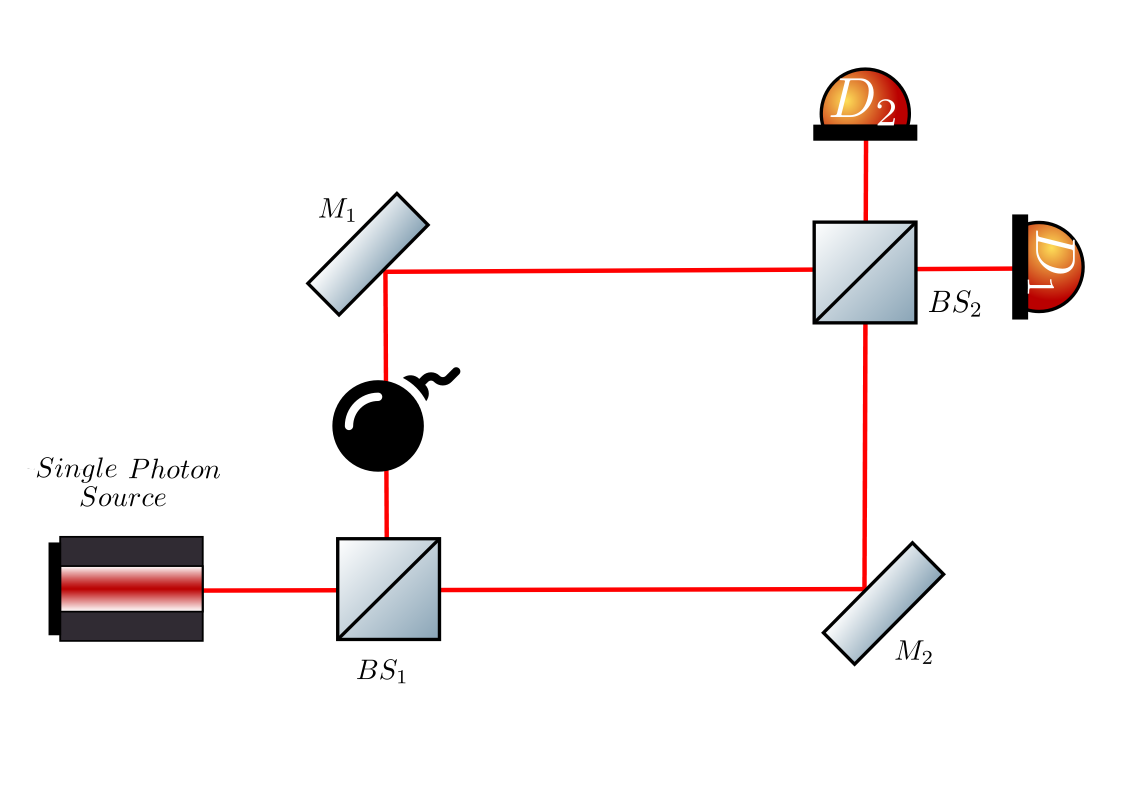
\includegraphics[width=\linewidth]{images/machzenhderbomb.png}
\caption{Elitzur-Vaidman's bomb detector}
\label{fig:BS2}
\end{figure}

To analyze this case we will simply repeat the calculations we did above this time having a perfect absorber in the vertical arm of the interferometer as Fig. 2 shows. We also need to consider that once the photon is absorbed the optical elements do not interact with it anymore. We will denote an absorbed photon using the $\ket{Abs}$ state. First, the initial state is transformed by the first $BS$ then the vertical path is absorbed by our perfect absorber then the state encounters mirrors and then if finally recombined in the second $BS$
  
\begin{align*}
&\ket{1}\xrightarrow{\text{BS1}}\cos(\theta_{1})\ket{1}+i\sin(\theta_{1})\ket{2}\\ &\xrightarrow{\text{Bomb}}\cos(\theta_{1})\ket{1}+i\sin(\theta_{1})\ket{Abs}\\ &\xrightarrow{\text{Mirrors}} 
 i\cos(\theta_{1})\ket{2}+i\sin(\theta_{1})\ket{Abs} \\ &\xrightarrow{\text{BS2}}i\cos(\theta_{1})\cos(\theta_{2})\ket{2}-\cos(\theta_{1})\sin(\theta_{2})\ket{1}+i\sin(\theta_{1})\ket{Abs} \numberthis
\end{align*}

The probabilities to be absorbed or detected at either $D_{1}$ or $D_{2}$ are given by :

\begin{align}
P_{D1}&=\cos^2(\theta_{1}) \sin^2(\theta_{2}) .\\
P_{D2}&=\cos^2(\theta_{1}) \cos^2(\theta_{2}).\\
P_{Abs}&=\sin^2(\theta_{1}).
\end{align}

Let us again consider the case where $\theta_{1}=\theta_{2}=\frac{\pi}{4}$ then:

\begin{equation}
P_{D1}=\frac{1}{4},\quad P_{D2}=\frac{1}{4}, \quad P_{Abs}=\frac{1}{2}.
\end{equation}

If the photon is detected at $D_{2}$ it would indicate that there's an object in one of the arms of the interferometer. This is often called non-interactive measurements because we can infer information about the object from the photons that did not interact with it. We cannot distinguish between this case and the previous one from a single event if we detect at $D_{1}$, so $\frac{1}{2}$ of the times we make a measurement we can't tell if a bomb is there or not.



\subsubsection{The single-photon Mach-Zehnder interferometer with an  \\ imperfect transmitter}

This section and the next ones are based on the treatment done by Z.Blanco and O.Rosas-Ortiz \cite{zuri} \cite{azuri} and the work done by Azuma \cite{Azuma}. Let us consider an object such that $\alpha'$ and $\beta'$ are its absorption and transmission coefficients, respectively, satisfying the condition $|\alpha|^2 + |\beta|^2 = 1.$.

We will use the same Horizontal-Vertical basis and our initial state $\ket{1}$. We will place our imperfect absorber in the vertical path. Our absorber can either transmit with probability $|\beta|^2$ or absorb with probability $|\alpha|^2$, such that when encountered with this object our states become:


\begin{align}
\ket{2}\xrightarrow[\text{Absorber}]{\text{Imperfect}}\alpha \ket{abs} +\beta \ket{2}.
\end{align}

With this information we can now go on with our calculations, First, the initial state goes through a $BS$, then it encounters our imperfect transmitter, after that it goes through a mirror in each path and then it is finally recombined in the second $BS$:

\begin{align*}
& \ket{1}\xrightarrow{\text{BS1}}\cos(\theta_{1})\ket{1}+i\sin(\theta_{1})\ket{2} \\ &\xrightarrow[\text{Absorber}]{\text{Imperfect }}\cos(\theta_{1})\ket{1}+i\sin(\theta_{1})(\alpha \ket{abs} +\beta \ket{2} )
\\ &\xrightarrow{\text{Mirrors}} i\cos(\theta_{1})\ket{2}+i \sin(\theta_{1})\alpha\ket{abs}-\sin(\theta_{1})\beta\ket{1} \\ &\xrightarrow{\text{BS2}} -
(\cos(\theta_{1})\sin(\theta_{2})+\beta \sin(\theta_{1})\cos(\theta_{2}))\ket{1}+ i \alpha \sin(\theta_{1})\ket{abs}+ \\ &i(\cos(\theta_{1})\cos(\theta_{2})-\sin(\theta_{1})\sin(\theta_{2})\beta)\ket{2}. \numberthis
\end{align*}


We will write detection probabilities as $P_{ij}$ where $i=1,2$ the path of the interferometer where the imperfect transmitter is placed, and $j$ is one of the possible outcomes, therefore the detection probabilities are given by:

\begin{align}
& P_{2D1}=|\cos(\theta_{1})\sin(\theta_{2})+\beta \sin(\theta_{1})\cos(\theta_{2})|^2. \\
& P_{2D2}=|\cos(\theta_{1})\cos(\theta_{2})-\beta \sin(\theta_{1})\sin(\theta_{2})|^2. \\
& P_{2abs}=|\alpha \sin(\theta_{1})|^2. 
\end{align}

If we consider the same procedure but this time we put our imperfect absorber on the horizontal arm of the interferometer we obtain:

\begin{align}
P_{1D1}&=|\cos(\theta_{1})\sin(\theta_{2})\beta +\sin(\theta_{1})\cos(\theta_{2})|^2. \\
P_{1D2}&=|\sin(\theta_{1})\sin(\theta_{2})-\beta \cos(\theta_{1})\cos(\theta_{2})|^2.\\
P_{1abs}&=|\alpha \cos(\theta_{1})|^2.
\end{align}



Observing the probabilities are different we can obtain the difference between them, expressions concerning the difference between $P_{D_{1}}$ and $P_{D_{2}}$ are important because they tell us just how distinguishable these outcomes are:


\begin{align}
P_{2D1}-P_{1D1}=(1-|\beta|^2)\left(\frac{\cos(2 \theta_{1})-\cos(2 \theta_{2})}{2}\right). \\
P_{2D2}-P_{1D2}=(1-|\beta|^2)\left(\frac{\cos(2 \theta_{1})+\cos(2 \theta_{2})}{2}\right).
\end{align}

From there, we can say that the probabilities are the same only when :

a)$\beta=1  $ which means a transparent object.

b)$\cos(2 \theta_{2})+\cos(2\theta_{1})=\cos(2 \theta_{1})-\cos(2\theta_{2})=0$   which means   $\theta_{1}=\theta_{2}=\frac{\pi}{4}\pm 2n\pi$
.

We can also obtain an expression for one of the angles in terms of the probabilities


\begin{align}
\theta_{2}=\frac{\cos^{-1}[\frac{(P_{1D2}-P_{2D2})-(P_{1D1}-P_{2D1})}{1-|\beta|^{2}}]}{2}.\\
\theta_{1}=\frac{\cos^{-1}[\frac{(P_{1D2}-P_{1D1})+(P_{1D1}-P_{2D1})}{1-|\beta|^{2}}]}{2}.
\end{align}


\pagebreak

\blankpage{}

\section{Mach-Zenhder interferometer with a beam \\ splitter as imperfect transmitter}

We will now study the case of a $BS$ as an imperfect transmitter. We consider imperfect mirrors such that $\gamma \neq 0$. We will see this is equivalent to including phase shifters in section 3.2 like in the previous cases we will first consider our imperfect transmitter in the vertical path as the Fig.4 shows, as we can see from the figure the reflected photon goes out of the interferometer's paths and therefore it's lost instead of being absorbed.

\begin{figure}[h!]
\centering
\includegraphics[width=\linewidth,height=7.5 cm]{images/machzenhderbs.png}
\caption{Mach-Zehnder interferometer with a BS as imperfect transmitter}
\label{fig:BS2}
\end{figure}

Our imperfect transmitter is a $BS$ whose transmission coefficient is $\cos(\theta_{o})$ and its reflection coefficient is $i\sin(\theta_{o})$. When a state interacts with our imperfect transmitter it becomes:

\begin{align}
\ket{2}\xrightarrow[\text{Absorber}]{\text{Imperfect}}i\sin(\theta_{o}) \ket{abs} +\cos(\theta_{o}) \ket{2}.
\end{align}

We consider the reflected photon to be lost since it goes out of our interferometer, and we denote that ``lost photon'' state by $\ket{abs}$, with that in mind now we can begin our calculation which is analogous to the ones from the previous sections:


\begin{align*}
&\ket{1}\xrightarrow{\text{BS1}}\cos(\theta_{1})\ket{1}+i\sin(\theta_{1})\ket{2}\xrightarrow{\text{BS}}\cos(\theta_{1})\ket{1}+i\sin(\theta_{1})(\cos(\theta_{o})\ket{2}+i\sin(\theta_{o})\ket{abs})\\ &\xrightarrow{\text{Mirrors}} \cos(\theta_{1})e^{i\gamma_{1}}\ket{2}+i\sin(\theta_{1})\cos(\theta_{o})e^{i\gamma_{2}}\ket{1}-\sin(\theta_{1})\sin(\theta_{o})\ket{abs}\\ &\xrightarrow{\text{BS2}}\cos(\theta_{1})e^{i\gamma_{1}}(\cos(\theta_{2})\ket{2}
+i\sin(\theta_{2})\ket{1})+i\sin(\theta_{1})\cos(\theta_{o})e^{i\gamma_{2}}(\cos(\theta_{2})\ket{1}+i\sin(\theta_{2})\ket{2})- \\ &\sin(\theta_{1})\sin(\theta_{o})\ket{abs}\\
&=(\cos(\theta_{1})e^{i\gamma_{1}}\cos(\theta_{2})-\sin(\theta_{1})\sin(\theta_{2})\cos(\theta_{o})e^{i\gamma_{2}})\ket{2}-\sin(\theta_{1})\sin(\theta_{o})\ket{abs}+\\ &(i\cos(\theta_{1})\sin(\theta_{2})e^{i\gamma_{1}}+ 
 i \sin(\theta_{1})\cos(\theta_{o})\cos(\theta_{2})e^{i\gamma_{2}})\ket{1}.\numberthis
\end{align*}



Detection probabilities are shown in Fig. 5, where we can see that for certain values of $\theta_{i}$ where $i=1,2,o$ the probabilities of detection in $D_{2}$ can be close to one:


\begin{figure}[t!]
\centering
\begin{subfigure}[b]{0.45\linewidth}
\includegraphics[width=\linewidth,height=2.8 cm]{images/P1abs.png}
\caption{$P_{2Abs}$}
\label{fig:BS2}
\end{subfigure}
\begin{subfigure}[b]{0.45\linewidth}
\includegraphics[width=\linewidth,height=2.8 cm]{images/P1d1.png}
\caption{$P_{2D1}$}
\label{fig:westminster_aerea}
\end{subfigure}
\begin{subfigure}[b]{0.45\linewidth}
\includegraphics[width=\linewidth,height=2.8 cm]{images/P1d2.png}
\caption{$P_{2D2}$}
\label{fig:BS2}
\end{subfigure}
\caption{Probability distributions with imperfect absorber in vertical path and $\theta_{o}=\frac{\pi}{3}$ y $\gamma_{2}-\gamma_{1}=\pi$.}
\label{fig:westminster}
\end{figure} 


\begin{align}
 P_{2D1}&=|ie^{i\gamma_{1}}\cos(\theta_{1})\sin(\theta_{2})+i e^{i\gamma_{2}}\cos(\theta_{o}) \sin(\theta_{1})\cos(\theta_{2})|^2.\\
 P_{2D2}&=|\cos(\theta_{1})\cos(\theta_{2})e^{i\gamma_{1}}- e^{i\gamma_{2}}\cos(\theta_{o}) \sin(\theta_{1})\sin(\theta_{2})|^2.\\
 P_{2Abs}&=|\sin(\theta_{o}) \sin(\theta_{1})|^2.
\end{align}


Repeating the same calculation with the object in the horizontal path we obtain the following probabilities, which are shown graphically in Fig. 6. We can see they are quite different and that is because we are always launching our photon from the same path, therefore, the situation is not symmetrical, that is the object isn't always in the same path the photon was sent into:


\begin{figure}[t!]
\centering
\begin{subfigure}[b]{0.45\linewidth}
\includegraphics[width=\linewidth]{images/P11abs.png}
\caption{$P_{1Abs}$}
\label{fig:BS1}
\end{subfigure}
\begin{subfigure}[b]{0.45\linewidth}
\includegraphics[width=\linewidth ,height=3 cm]{images/P11d1.png}
\caption{$P_{1D1}$}
\label{fig:westminster_aerea}
\end{subfigure}
\begin{subfigure}[b]{0.45\linewidth}
\includegraphics[width=\linewidth]{images/P11d2.png}
\caption{$P_{1D1}$}
\label{fig:BS1}
\end{subfigure}
\caption{Probabilities distribution in the Horizontal path for $\theta_{o}=\frac{\pi}{3}$ y $\gamma_{2}-\gamma_{1}=\pi$}
\label{fig:westminster}
\end{figure} 



\begin{align}
P_{1D1}&=|ie^{i\gamma_{1}}\cos(\theta_{1})\sin(\theta_{2})\cos(\theta_{o})+i e^{i\gamma_{2}}\sin(\theta_{1})\cos(\theta_{2})|^2. \\
P_{1D2}&=|\cos(\theta_{1})\cos(\theta_{o})\cos(\theta_{2})e^{i\gamma_{1}}-e^{i\gamma_{2}} \sin(\theta_{1})\sin(\theta_{2})|^2.\\
P_{1Abs}&=|\sin(\theta_{o}) \cos(\theta_{1})|^2.
\end{align}


This analysis is totally consistent with Zurika's \cite{zuri} when one takes the case $\beta'=\cos(\theta_{o})$, $\alpha'=i \sin(\theta_{o})$ and $\gamma_{2}-\gamma_{1}=0$. However this case has a little advantage and that is that our ``absorbed'' photon, is not absorbed but goes out of our interferometer so we can measure all outputs of the interferometer by placing a detector, say $D_{abs}$, in the path the ``lost photon" would follow.

\subsection{$N$ Beam Splitters as imperfect absorber }
\vspace{1 cm}


\begin{figure}[hbt!]
\centering
\includegraphics[width=\linewidth,height=8 cm]{images/machzenhderBSS.png}
\caption{Mach Zehnder with $N$ BS as imperfect absorber}
\label{fig:BS2}
\end{figure}


We begin analyzing what happens if our initial state goes through several BS assuming the reflected photon is ``lost". We will study both initial states in parallel, as Fig.7 shows. We are placing N beams splitters in one of the paths of the interferometer so:

\begin{align}
BS_{1}\ket{1}=\cos(\theta_{1})\ket{1}+i\sin(\theta_{1})\ket{abs}.\\
BS_{1}\ket{2}=\cos(\theta_{1})\ket{2}+i\sin(\theta_{1})\ket{abs}.
\end{align}

The next BS only acts on the transmitted photon so:
\begin{align}
&BS_{2}(\cos(\theta_{1})\ket{1}+i\sin(\theta_{1})\ket{abs})=\cos(\theta_{1})BS_{2}\ket{1}+i\sin(\theta_{1})\ket{abs}.\\
&BS_{2}(\cos(\theta_{1})\ket{2}+i\sin(\theta_{1})\ket{abs})=\cos(\theta_{1})BS_{2}\ket{2}+i\sin(\theta_{1})\ket{abs}.\\
&BS_{2}BS_{1}\ket{2}=\cos(\theta_{1})\cos(\theta_{2})\ket{2}+i A'\ket{abs}.\\
&BS_{2}BS_{1}\ket{1}=\cos(\theta_{1})\cos(\theta_{2})\ket{1}+i A\ket{abs}.
\end{align}
Then, the next BS does the same

\begin{align}
BS_{3}BS_{2}BS_{1}\ket{1}=\cos(\theta_{1})\cos(\theta_{2})\cos(\theta_{3})\ket{1}+iB\ket{abs}.\\
BS_{3}BS_{2}BS_{1}\ket{2}=\cos(\theta_{1})\cos(\theta_{2})\cos(\theta_{3})\ket{2}+iB'\ket{abs}.
\end{align}
so after n BS :

\begin{align}
BS^{n}=BS_{n}...BS_{3}BS_{2}BS_{1}\ket{1}=\cos(\theta_{1})\cos(\theta_{2})\cos(\theta_{3})....\cos(\theta_{n})\ket{1}+i C\ket{abs}.\\
BS^{n}=BS_{n}...BS_{3}BS_{2}BS_{1}\ket{2}=\cos(\theta_{1})\cos(\theta_{2})\cos(\theta_{3})....\cos(\theta_{n})\ket{2}+i C'\ket{abs}.
\end{align}

We can obtain $C$ and $C'$ by asking the probabilities to add to unity, since everything that is not transmitted will be ``lost":

\begin{align}
BS^{n}\ket{1}&=\prod_{i=1}^{n} \cos(\theta_{i})\ket{1}+i D\ket{abs}.\\
BS^{n}\ket{2}&=\prod_{i=1}^{n} \cos(\theta_{i})\ket{2}+i D'\ket{abs}.\\
D'=D&=\sqrt{1-\prod_{i=1}^{n}\cos^2(\theta_{i})}
\end{align}

We now use this as a imperfect absorber in the vertical path:

\begin{align*}
&\ket{1}\xrightarrow{\text{BS1}}\cos(\theta_{1})\ket{1}+i\sin(\theta_{1})\ket{2}\\ &\xrightarrow{{B^{n}}}\cos(\theta_{1})\ket{1}+i\sin(\theta_{1})\prod_{i=3}^{n} \cos(\theta_{i})\ket{2}-\sin(\theta_{1})\sqrt{1-\prod_{i=3}^{n}\cos^2(\theta_{i})}\ket{Abs} \\ & \xrightarrow{{Mirrors}}\cos(\theta_{1})  e^{i \gamma_{1}}\ket{2}+i\sin(\theta_{1})\prod_{i=3}^{n} \cos(\theta_{i}) e^{i \gamma_{2}}\ket{1}-\sin(\theta_{1})\sqrt{1-\prod_{i=3}^{n}\cos^2(\theta_{i})}\ket{Abs} \\ & \xrightarrow{{BS2}}(\cos(\theta_{1})\cos(\theta_{2})e^{i \gamma_{1}}-\sin(\theta_{1})\sin(\theta_{2})e^{i \gamma_{2}}\prod_{i=3}^{n} \cos(\theta_{i}))\ket{2}+\\ & i(\cos(\theta_{1})\sin(\theta_{2})e^{i \gamma_{1}}+\cos(\theta_{2})\sin(\theta_{1})e^{i \gamma_{2}}\prod_{i=3}^{n} \cos(\theta_{i}))\ket{1}-\sin(\theta_{1})\sqrt{1-\prod_{i=3}^{n}\cos^2(\theta_{i})}\ket{Abs}.
\end{align*}
 
The probabilities of detection in each of the detectors are given by:

\begin{align}
P_{D1}&=|\cos(\theta_{1})\sin(\theta_{2})e^{i \gamma_{1}}+\cos(\theta_{2})\sin(\theta_{1})e^{i \gamma_{2}}\prod_{i=3}^{n} \cos(\theta_{i})|^2.\\
P_{D2}&=|\cos(\theta_{1})\cos(\theta_{2})e^{i \gamma_{1}}-\sin(\theta_{1})\sin(\theta_{2})e^{i \gamma_{2}}\prod_{i=3}^{n} \cos(\theta_{i})|^2.\\
P_{Abs}&=\sin^2(\theta_{1})\left(1-\prod_{i=3}^{n}\cos^2(\theta_{i})\right).
\end{align}

\subsection{Analysis with phase retarders }

The interferometer is an instrument quite hard to align experimentally, in most cases alignment is a little off. We can characterize just how off this alignment is by considering the effects of phase retarders on the interferometer after all misalignment is nothing but differences in the optical path. Those predictions can be compared with the actual interferometer (without phase retarders), a wave retarder's  matrix representation is:


\begin{equation}
 Retarder=\begin
{pmatrix} e^
{i c} & 0\\0& e^
{i k }\end
{pmatrix}
\end{equation}.

Let's see the effect of such an optical device in our setup:
\begin{align*}
&\ket{1}\xrightarrow{\text{BS1}}\cos(\theta_{1})\ket{1}+i\sin(\theta_{1})\ket{2}\\ &\xrightarrow[\text{Absorber}]{\text{Imperfect }}cos(\theta_{1})\ket{1}+i\sin(\theta_{1})(\alpha' \ket{abs} +\beta' \ket{2} )\\& \xrightarrow[\text{Retarders}]{\text{Phase}}\cos(\theta_{1})e^{ic}\ket{1}+i\beta'\sin(\theta_{1}) e^{ik}\ket{2} +i\alpha'\sin(\theta_{1}) \ket{abs}\\ &\xrightarrow{\text{Mirrors}} \cos(\theta_{1})e^{i(\gamma_{1}'+c)}\ket{2}+i \sin(\theta_{1})\alpha'\ket{abs}+i\sin(\theta_{1})\beta'e^{i(\gamma_{2}'+k)}\ket{1},
\end{align*}

we can stop here by noticing that making $\gamma_{2}'+k=\gamma_{2}$ and $\gamma_{1}'+c=\gamma_{1}$ we have the exact same case as in our previous sections, like in the section of a BS as an imperfect absorber with  $\beta=cos(\theta_{o})$ and $\alpha=i\sin(\theta_{o})$ so our model that makes use of the general matrix of a mirror instead of using the more popular perfect mirror matrix $M=\begin{pmatrix} i & 0\\0& i\end{pmatrix}$, where $i=e^{i \frac{\pi}{2}}=\gamma$, has the  effect of a phase retarder included, allowing us to study misalignment.
 
\pagebreak

\section{Optical chopper as perfect absorber }
 
 \begin{figure}[h!]
\centering
\includegraphics[width=\linewidth]{images/machzenhderchopper.png}
\caption{Mach-Zehnder with an optical chopper as an imperfect absorber}
\label{fig:BS2}
\end{figure}
An optical chopper is a device that periodically interrupts light. It is usually a disk with holes rotating with a certain frequency (which can vary in time) from its definition we can infer that it can be modeled using a square wave which can be written as  $f(t)=\frac{sgn(\sin(wt))+1}{2}$, where $\omega$ is the angular frequency of the optical chopper multiplied by the number of ``hole-material" pairs which for now we assume are the same size. 
  
We will be ignoring diffraction effects, a consequence of modeling it like this is that consecutive optical choppers become the product of square waves and products of square waves is again a square wave, so modeling many choppers would be the same as modeling one with that effective frequency, as Fig.8 shows. In this section we intend to analyze the Mach-Zehnder interferometer with a chopper being the imperfect absorber, the chopper introduces a discrete-time dependence, therefore we will be alternating between two different probability distributions.


We can model our optical chopper by using an operator $C_{i}$ where $i$ is the path where the chopper is placed, such that in our base(where $i=1,2$ and $i \neq j$):

\begin{align}
C_{i}\ket{i}&=f(t)\ket{i}.\\
C_{j}\ket{i}&=\ket{i}.
\end{align}

Ideally, we want this operator to be unitary in the ``hole" cycle. Since we are modeling the whole as a transparent object. This will be checked right away:

\begin{equation}
|f|^2=\frac{(sgn(\sin(wt)+1)^2}{4},
\end{equation}
the sign function squared is always one so
\begin{align}
&|f|^2=\frac{2(1+sgn(\sin(wt)))}{4}. \\
&|f|^2=f,
\end{align}


from there we can see that it is a unitary matrix whenever the sine is in the positive cycle, and it becomes null in the negative cycle, that happens because in the negative cycle we have total absorption. The absorption coefficient would  be:  

\begin{align}
 a&=1-f.\\
 a&=\frac{1-sgn(\sin(wt))}{2}.\\
|a|^2&=\frac{2(1-sgn(\sin(wt)))}{4}.\\
|a|^2&=a.
\end{align}

We will now analyze a Mach-Zehnder interferometer using a chopper as a time-dependent absorber. The chopper will be placed on the vertical path, and our photon will go into the interferometer using the horizontal path



\begin{align*}
&\ket{1}\xrightarrow{\text{BS1}}\cos(\theta_{1})\ket{1}+i\sin(\theta_{1})\ket{2}\\ &\xrightarrow{\text{Chopper}}\cos(\theta_{1})\ket{1}+i\sin(\theta_{1})f\ket{2}+i\sin(\theta_{1})a\ket{abs}\\ &\xrightarrow{\text{Mirrors}} \cos(\theta_{1})e^{i\gamma_{1}}\ket{2}+i\sin(\theta_{1})f e^{i\gamma_{2}}\ket{1}+i\sin(\theta_{1})a\ket{abs}\\& \xrightarrow{\text{BS2}}\cos(\theta_{1})e^{i\gamma_{1}}(\cos(\theta_{2})\ket{2}+i\sin(\theta_{2})\ket{1})+i\sin(\theta_{1})e^{i\gamma_{2}}f(\cos(\theta_{2})\ket{1}+i\sin(\theta_{2})\ket{2})+i\sin(\theta_{1})a\ket{abs}\\
& = i(e^{i\gamma_{1}}\cos(\theta_{1})\sin(\theta_{2})+f e^{i\gamma_{2}}\sin(\theta_{1})\cos(\theta_{2}))\ket{1}+(\cos(\theta_{1})\cos(\theta_{2}) e^{i\gamma_{1}}- \\&  \sin(\theta_{1})\sin(\theta_{2})f e^{i \gamma_{2}})\ket{2}+i\sin(\theta_{1})a\ket{abs}. \numberthis
\end{align*} 



A plot for the detection probabilities is shown in Fig.9, as we mentioned before the system is alternating between two probability distributions. We can see those for each of the possible states in the figure. It is worth noting that the absorption graph alternates between the one shown and no absorption: 



\begin{figure}[t!]
\centering

\begin{subfigure}[b]{0.45\linewidth}
\includegraphics[width=\linewidth,height=3 cm]{images/Pc2Abs.png}
\caption{$P_{1Abs}$}
\label{fig:BS1}
\end{subfigure}
\begin{subfigure}[b]{0.45\linewidth}
\includegraphics[width=\linewidth,,height=3 cm]{images/Pc2D21.png}
\caption{$P_{2D2}$ in the first cycle }
\label{fig:BS1}
\end{subfigure}
\begin{subfigure}[b]{0.45\linewidth}
\includegraphics[width=\linewidth,height=3 cm]{images/Pc2D22.png}
\caption{$P_{2D2}$ in the second cycle}
\label{fig:BS1}
\end{subfigure}
\begin{subfigure}[b]{0.45\linewidth}
\includegraphics[width=\linewidth,height=3 cm]{images/Pc2D11.png}
\caption{$P_{2D1} $ in the first cycle}
\label{fig:westminster_aerea}
\end{subfigure}
\begin{subfigure}[b]{0.45\linewidth}
\includegraphics[width=\linewidth,height=3 cm]{images/Pc2D12.png}
\caption{$P_{2D1} $ in the second cycle }
\label{fig:BS1}
\end{subfigure}
\caption{Probability Distribution for $\gamma_{2}-\gamma_{1}=\frac{\pi}{2}$ in the vertical path}
\label{fig:westminster}
\end{figure}


\begin{align}
&P_{2D1}=|e^{i\gamma_{1}}\cos(\theta_{1})\sin(\theta_{2})+f e^{i\gamma_{2}}\sin(\theta_{1})\cos(\theta_{2})|^2.\\
&P_{2D2}=|\cos(\theta_{1})\cos(\theta_{2})e^{i\gamma_{1}}- f \sin(\theta_{1})\sin(\theta_{2})e^{i\gamma_{2}}|^2.\\
&P_{2Abs}=|a \sin(\theta_{1})|^2.
\end{align}

Which can be rewritten as:
\begin{align}
& P_{2D1}=\cos^2(\theta_{1})\sin^2(\theta_{2})+f^2 \sin^2(\theta_{1})\cos^2(\theta_{2})+\frac{f \sin(2\theta_{1})\sin(2\theta_{2})\cos(\gamma_{1}-\gamma_{2})}{2}.\\
& P_{2D2}=\cos^2(\theta_{1})\cos^2(\theta_{2})+ f^2 \sin^2(\theta_{1})\sin^2(\theta_{2})-\frac{f \sin(2\theta_{1})\sin(2\theta_{2})\cos(\gamma_{1}-\gamma_{2})}{2}.\\
& P_{2Abs}=a^2 \sin^2(\theta_{1}).
\end{align}

By the same procedure having the chopper in the horizontal path, one can obtain the following results which are shown in Fig.9, for each of the possible states of the system
 
\begin{figure}[h!]
\centering
\begin{subfigure}[b]{0.35\linewidth}
\includegraphics[width=\linewidth,height=3 cm]{images/Pc1Abs.png}
\caption{$P_{1Abs}$}
\label{fig:BS1}
\end{subfigure}
\begin{subfigure}[b]{0.35\linewidth}
\includegraphics[width=\linewidth,height=3 cm]{images/Pc1D21.png}
\caption{$P_{1D2}$ in the first cycle }
\label{fig:BS1}
\end{subfigure}
\begin{subfigure}[b]{0.35\linewidth}
\includegraphics[width=\linewidth,height=3 cm]{images/Pc1D22.png}
\caption{$P_{1D2}$ in the second cycle}
\label{fig:BS1}
\end{subfigure}
\begin{subfigure}[b]{0.35\linewidth}
\includegraphics[width=\linewidth,height=3 cm]{images/Pc1D11.png}
\caption{$P_{1D1} $ in the first cycle}
\label{fig:westminster_aerea}
\end{subfigure}
\begin{subfigure}[b]{0.35\linewidth}
\includegraphics[width=\linewidth,height=3 cm]{images/Pc1D12.png}
\caption{$P_{1D1} $in the second cycle }
\label{fig:BS1}
\end{subfigure}
\caption{Probability distribution for the horizontal path and  $\gamma_{2}-\gamma_{1}=\frac{\pi}{2}$}
\label{fig:westminster}
\end{figure}

\begin{align}
& P_{1D1}=\cos^2(\theta_{1})\sin^2(\theta_{2})f^2+ \sin^2(\theta_{1})\cos^2(\theta_{2})+\frac{f \sin(2\theta_{1})\sin(2\theta_{2})\cos(\gamma_{1}-\gamma_{2})}{2}.\\
& P_{1D2}=\cos^2(\theta_{1})\cos^2(\theta_{2})f^2+ \sin^2(\theta_{1})\sin^2(\theta_{2})-\frac{f \sin(2\theta_{1})\sin(2\theta_{2})\cos(\gamma_{1}-\gamma_{2})}{2}.\\
& P_{2Abs}=a^2 \cos^2(\theta_{1}).
\end{align}

Since $f^2=f$, we can write the difference of probabilities as:

\begin{align}
P_{1D1}-P_{1D2}=(a)\left(\frac{\cos(2 \theta_{1})-\cos(2 \theta_{2})}{2}\right).\\
P_{2D1}-P_{2D2}=(a)\left(\frac{\cos(2 \theta_{1})+\cos(2 \theta_{2})}{2}\right).
\end{align}
 From there we can obtain either $\theta_{1}$  or $\theta_{2}$ :
\begin{align}
&(P_{1D1}-P_{1D2})+(P_{2D1}-P_{2D2})=(a)(\cos(2 \theta_{1})).\\
&(P_{1D1}-P_{1D2})-(P_{2D1}-P_{2D2})=(-a)(\cos(2 \theta_{2})).\\
 &\theta_{1}=\frac{1}{2}\cos^{-1}\left[\frac{(P_{1D1}-P_{1D2})+(P_{2D1}-P_{2D2})}{a}\right].\\
 &\theta_{2}=\frac{1}{2}\cos^{-1}\left[\frac{(P_{1D1}-P_{1D2})-(P_{2D1}-P_{2D2})}{a}\right].
 \end{align}
 
\pagebreak

\subsection{Optical chopper as imperfect absorber}

Previously we considered the ``material" part of the chopper as a perfect absorber. In this section we will now generalize to when it is an imperfect absorber, this can be done quite simply by defining :
 

\begin{align} 
f_{hole}&=\frac{1+sgn(\sin(wt))}{2}.\\
f_{material}&=\left(\frac{1-sgn(\sin(wt))}{2} \right)\beta.\\
f&=f_{material}+f_{hole}.
\end{align}


Where $\beta$ is the transmission coefficient of the material part of our chopper, $\beta$ could be a function of  $\omega$ or t in this analysis. The operator used to describe our chopper is the same as in the previous section, we define:

\vspace{0.5cm}
\begin{equation}
a=\left(\frac{1-sgn(\sin(wt))}{2}\right) \alpha.
\end{equation}
\vspace{0.5cm}

Where $\alpha$ is the absorption coefficient of the material part of our chopper, by using this notation we have the same case as in the previous section, except this time $f^2 \neq 1$ :

\begin{align}
|a|^2&=a \alpha.\\
|f_{material}|^2&=f_{material} \beta,
\end{align}

which we can generalize to obtain:

\begin{align}
|a|^n&=a\alpha^{n-1}.\\
|f_{material}|^n&=f_{material} \beta^{n-1},
\end{align}
so we have:

\begin{equation}
|f|^2=  \frac{\abs{\alpha}^2}{2} sgn(\sin(wt)) +\frac{1+\abs{\beta}^2}{2}.
\end{equation}



Substituting in the previous section yields the probability distributions shown in Fig.11:
\begin{figure}[h]
\centering
\begin{subfigure}[b]{0.40\linewidth}
\includegraphics[width=\linewidth,height=3 cm]{images/p1cabs.png}
\caption{$P_{1Abs}$}
\label{fig:BS1}
\end{subfigure}
\begin{subfigure}[b]{0.40\linewidth}
\includegraphics[width=\linewidth,height=3 cm]{images/p1cd21.png}
\caption{$P_{1D2}$ in the first cycle }
\label{fig:BS1}
\end{subfigure}
\begin{subfigure}[b]{0.40\linewidth}
\includegraphics[width=\linewidth,height=3 cm]{images/p1cd22.png}
\caption{$P_{1D2}$ in the second cycle}
\label{fig:BS1}
\end{subfigure}
\begin{subfigure}[b]{0.40\linewidth}
\includegraphics[width=\linewidth,height=3 cm]{images/p1cd11.png}
\caption{$P_{1D1} $ in the first cycle}
\label{fig:westminster_aerea}
\end{subfigure}
\begin{subfigure}[b]{0.40\linewidth}
\includegraphics[width=\linewidth,height=3 cm]{images/p1cd12.png}
\caption{$P_{1D1} $ in the second cycle }
\label{fig:BS1}
\end{subfigure}
\caption{Probability Distribution in the horizontal path with  $\gamma_{2}-\gamma_{1}=0 $ y $\beta=0.5$}
\label{fig:westminster}
\end{figure}


\begin{align}
&P_{1D1}=\cos^2(\theta_{1})\sin^2(\theta_{2})\abs{f}^2+ \sin^2(\theta_{1})\cos^2(\theta_{2})+\frac{\Re{f} \sin(2\theta_{1})\sin(2\theta_{2})\cos(\gamma_{1}-\gamma_{2})}{2}.\\
&P_{1D2}=\cos^2(\theta_{1})\cos^2(\theta_{2})\abs{f}^2+ \sin^2(\theta_{1})\sin^2(\theta_{2})-\frac{\Re{f} \sin(2\theta_{1})\sin(2\theta_{2})\cos(\gamma_{1}-\gamma_{2})}{2}.\\
&P_{1Abs}=\abs{\alpha}^2 \cos^2(\theta_{1}).
\end{align}


When the optical chopper is in the vertical path we obtain the following detection probabilities. The probability distributions are shown in Fig.12:

\begin{figure}[!h]
\centering
\begin{subfigure}[b]{0.40\linewidth}
\includegraphics[width=\linewidth,height=3 cm]{images/pcabs.png}
\caption{$P_{1Abs}$}
\label{fig:BS1}
\end{subfigure}
\begin{subfigure}[b]{0.40\linewidth}
\includegraphics[width=\linewidth,height=3 cm]{images/pcd21.png}
\caption{$P_{2D1}$ in the first cycle }
\label{fig:BS1}
\end{subfigure}
\begin{subfigure}[b]{0.40\linewidth}
\includegraphics[width=\linewidth,height=3 cm]{images/pcd22.png}
\caption{$P_{2D1}$ in the second cycle}
\label{fig:BS1}
\end{subfigure}
\begin{subfigure}[b]{0.40\linewidth}
\includegraphics[width=\linewidth,height=3 cm]{images/pcd11.png}
\caption{$P_{2D1} $ in the first cycle}
\label{fig:westminster_aerea}
\end{subfigure}
\begin{subfigure}[b]{0.40\linewidth}
\includegraphics[width=\linewidth,height=3 cm]{images/pcd12.png}
\caption{$P_{2D1} $ in the second cycle }
\label{fig:BS1}
\end{subfigure}
\caption{Probability Distribution for the vertical path with  $\gamma_{2}-\gamma_{1}=0 $ y $\beta=0.5$}
\label{fig:westminster}
\end{figure}

\begin{align}
&P_{2D1}=\cos^2(\theta_{1})\sin^2(\theta_{2})+\abs{f}^2 \sin^2(\theta_{1})\cos^2(\theta_{2})+\frac{\Re{f} \sin(2\theta_{1})\sin(2\theta_{2})\cos(\gamma_{1}-\gamma_{2})}{2}.\\
&P_{2D2}=\cos^2(\theta_{1})\cos^2(\theta_{2})+ \abs{f}^2 \sin^2(\theta_{1})\sin^2(\theta_{2})-\frac{\Re{f} \sin(2\theta_{1})\sin(2\theta_{2})\cos(\gamma_{1}-\gamma_{2})}{2}.\\
&P_{2Abs}=\abs{\alpha}^2 \sin^2(\theta_{1}).
\end{align}



\newpage


\section{Analysis of $N$ intereferometers }
 
 The notation previously used is not popular when dealing with nested interferometers. To be consistent with the existing literature we will use the same notation as Kwait et al.\cite{5}, where we have an interferometer  like the one in the following Fig.13, we see from the figure that we will have $N$ $BS$ and $N-1$ Absorbers:
 
\begin{figure}[!htb]
\centering
\includegraphics[width=\linewidth]{images/nmach.png}
\caption{Nested Mach-Zehnders  with imperfect absorbers}
\label{fig:BS2}
\end{figure}
 
 We will still use a binary basis, but instead of using the Horizontal-Vertical, it will be a path A-path B basis. That is an ``up-down" basis, we will use $\ket{2}$ for path $b$ and $\ket{1}$ for path $a$, one of the main advantages of this basis is that the mirror matrices are diagonal because they keep our photon on the same path. We will model our imperfect absorber using a non-unitary diagonal matrix just as was done by  Azuma \cite{Azuma}.   
 
 Azuma used a matrix of the form, where $n=\abs{\beta}^{2}$:
 
 \begin{equation}
 A_{Azuma}=\begin{pmatrix} \sqrt{n} & 0\\0& 1\end{pmatrix}.
 \end{equation}

Since we are using a $BS$ as an imperfect absorber a more suitable option would be :
\begin{equation}
 A_{BS}=\begin{pmatrix} \cos(\theta) & 0\\0& 1\end{pmatrix}.
\end{equation}

The final state can be obtained by applying all of the operators to the initial state which will be $\ket{2}$, Let us first consider that we have no imperfect absorbers on the interferometer, then the only operators acting on the state are $BS$ then:

\begin{align}
&BS_{i} \times BS_{i+1}=\begin{pmatrix} \cos(\theta_{i}) & i \sin(\theta_{i}) \\ i \sin(\theta_{i}) & \cos(\theta_{i}) \end{pmatrix}  
\begin{pmatrix} \cos(\theta_{i+1}) & i \sin(\theta_{i+1}) \\ i \sin(\theta_{i+1}) & \cos(\theta_{i+1}) \end{pmatrix}.\\
&=\begin{pmatrix} \cos(\theta_{i})\cos(\theta_{i+1})-\sin(\theta_{i})\sin(\theta_{i+1}) & i (\cos(\theta_{i+1})\sin(\theta_{i})+\cos(\theta_{i})\sin(\theta_{i+1})) \\ i (\cos(\theta_{i+1})\sin(\theta_{i})+\cos(\theta_{i})\sin(\theta_{i+1}))& \cos(\theta_{i})\cos(\theta_{i+1})-\sin(\theta_{i})\sin(\theta_{i+1}) \end{pmatrix}.\\ 
&=\begin{pmatrix} \cos(\theta_{i}+\theta_{i+1}) & i \sin(\theta_{i}+\theta_{i+1}) \\ i \sin(\theta_{i}+\theta_{i+1}) & \cos(\theta_{i}+\theta_{i+1}) \end{pmatrix},
\end{align}

if we assume $N$ $BS$ that are identical:

\begin{equation}
BS^{N}=\begin{pmatrix} \cos(N\theta) & i \sin(N\theta) \\ i \sin(N\theta) & \cos(N\theta) \end{pmatrix}
\end{equation}

Let's assume $\theta=\frac{\pi}{2N}$ so we have:

\begin{equation}
BS^{N}=\begin{pmatrix} 0 & i  \\ i  & 0 \end{pmatrix},
\end{equation}

so we will always detect the photon in the path that is not the one we sent our photon in, with this in mind let us see what happens with this particular $\theta$ when we do have imperfect absorbers. The state first goes through a BS, then one of the imperfect absorbers and then another BS, it keeps going like that until it encounters the $Nth$ and last $BS$. We have $N$ $BS$ and $N-1$ imperfect absorbers so our final state is:


\begin{equation}\ket{2}\xrightarrow[\text{interferometers}]{\text{Nested}}(B \times A)^{N-1}B \ket{2}.
\end{equation}

Detection probabilities are given by:

\begin{align}
&P_{D1}=|\bra{2} (B \times A)^{N-1}B \ket{2}|^2.\\
&P_{D2}=|\bra{1} (B \times A)^{N-1}B \ket{2}|^2.\\
&P_{Abs}=1-P_{D1}-P_{D2}.
\end{align}
 
 
To obtain said probabilities as well as the behavior of the system for varying $N$ we will make use of a computer. The program was written in python and yielded the following results:


 
\begin{figure}[h]
\centering
\begin{subfigure}[b]{0.3\linewidth}
\includegraphics[width=\linewidth,height=5 cm]{images/BS_Azuna.png}
\caption{$P_{D1}$}
\label{fig:BS1}
\end{subfigure}
\begin{subfigure}[b]{0.3\linewidth}
\includegraphics[width=\linewidth,height=5 cm]{images/BS_AzunaD2.png}
\caption{$P_{D2}$}
\label{fig:westminster_aerea}
\end{subfigure}
\begin{subfigure}[b]{0.3\linewidth}
\includegraphics[width=\linewidth,height=5 cm]{images/absorbido_azuna.png}
\caption{$P_{D2}$}
\label{fig:BS1}
\end{subfigure}
\caption{Probabilities when BS is an imperfect absorber, D1 is in path b, and D2 in path a}
\label{Bs n imperfect}
\end{figure} 


Fig. \ref{Bs n imperfect} shows the different probabilities for absorption, and detection as we increase $N$. We can see this asymptotically approaches one as Azuma had shown \cite{Azuma}, the case of a $BS$ as an absorber shows consistency. This is important because the case of a $BS$ is described by the same mathematics that and analyzer and a polarizer \cite{Leonhardt_2003} and unlike other absorbers this can be manipulated continually, giving us a way to test this curves experimentally.
 
One may wonder how the system behaves for growing $N$ with the same kind of $BS$ for all $N$, maybe we could make the probabilities grow as well, but after the analysis. We can see that even though it grows for low N it soon begins to lower and approaches 0 very quickly for most values as we can see below. 




\begin{figure}[!htb]
\centering
\begin{subfigure}[b]{0.45\linewidth}
\includegraphics[width=\linewidth]{images/BsFijo_azumaD1.png}
\caption{$P_{D1}$}
\label{fig:BS1}
\end{subfigure}
\begin{subfigure}[b]{0.45\linewidth}
\includegraphics[width=\linewidth]{images/BsFijo_azumaD2.png}
\caption{$P_{D2}$}
\label{fig:westminster_aerea}
\end{subfigure}
\begin{subfigure}[b]{0.45\linewidth}
\includegraphics[width=\linewidth]{images/BsFijo_azumaabs.png}
\caption{$P_{D2}$}
\label{fig:BS1}
\end{subfigure}
\caption{Behavior for growing N 50/50 BS for all N}
\label{growing 50/50}
\end{figure} 
 
 Fig. \ref{growing 50/50} shows the probabilities when we increase the number of interferometers but do not change the value of the $BS$ as $N$ increases, this may seem like a waste of effort since the aim is to maximize the detection probability. However let us assume that we have an absorber that has a very little absorption probability, if we wanted to have it absorbing our photon this scheme would prove useful

\subsection{Optical chopper as imperfect absorber in $N$ interferometers}
For an optical chopper the following matrix could be used:

\begin{equation}
A_{chopper}=\begin{pmatrix} f & 0 \\ 0 & 1 \end{pmatrix}.
\end{equation}

However as f only varies discretely our matrix will alternate between two values of $n$,between two transparencies :

\begin{equation}
f=\left(\frac{1-sgn(\sin(wt))}{2} \right)\beta+\frac{1+sgn(\sin(wt))}{2}.
\end{equation}

in the positive cycle we have $f_{positive}=1$. While on the negative cycle $f_{negative}=\beta$. For convenience, we will redefine $n=\abs{\beta}^{2}$ and write in terms of $n$, this way in the positive cycle we will have the case of the nested interferometer with no object which is the same as  $\beta=1$, but in the negative cycle, we will have  Azuma's case. We now use Azuma's matrix to perform the same analysis and also realize the probabilities will alternate between the blue line $\beta=1$ and the line which is $\beta=Transmittance$ of our chopper:


 \begin{figure}[!htb]
\centering
\begin{subfigure}[b]{0.45\linewidth}
\includegraphics[width=\linewidth]{images/ChopperD1.png}
\caption{$P_{D1}$}
\label{fig:BS1}
\end{subfigure}
\begin{subfigure}[b]{0.45\linewidth}
\includegraphics[width=\linewidth]{images/ChopperD2.png}
\caption{$P_{D2}$}
\label{fig:westminster_aerea}
\end{subfigure}
\begin{subfigure}[b]{0.45\linewidth}
\includegraphics[width=\linewidth]{images/Chopper_abs.png}
\caption{$P_{D2}$}
\label{fig:BS1}
\end{subfigure}
\caption{Behavior for Growing N for a chopper as imperfect absorbers}
\label{n chopper}
\end{figure}
 
\vspace{5 cm}

Fig. \ref{n chopper} shows the probabilities of a given absorber, the blue line represents the ``hole" part of the chopper, and the other lines represent the ``material" part, the system will alternate periodically between these probabilities

\pagebreak

\section{Experimental Setup}
In this chapter, we will describe the necessary materials and steps to realize all of the previous content of this thesis experimentally. All of the work from this section on took place at the laboratory for quantum and electromagnetic phenomena at UPIITA. We will begin by generating a single photon source using SPDC, we will follow the approach taken in \cite{maestria_procopio}. We will then replicate the Elitzur-Vaidman ``bomb detector''. Finally, we will study variations of this ``bomb detector'' with semitransparent objects.

\subsection{Single photon source}

To produce a single-photon source we will use the SPDC process described in chapter 1, to do this experimentally we will follow the method described in \cite{maestria_procopio}. The experimental setup can be seen in Fig. \ref{single}.  We will use the following materials:

\begin{figure}[!htb]
\centering
\includegraphics[width=\linewidth]{images/SPDC_exp.png}
\caption{Experimental setup of single photon source}
\label{single}
\end{figure}



\begin{itemize}

\item Aluminum rails
\item Infrared filters 810nm ± 10nm
\item Violet laser 405nm
\item Pinholes
\item BBO-I crystal
\item Multimode optical fiber
\item APDs(Avalanche photo-diodes)
\item National instruments' data acquisition board 
\item Newport posts
\item Optical Table

\end{itemize}

The first step to achieve a single photon source is to find the most likely light-cone using individual counts in each photo-detector as described in chapter 2 section 2.1 where we explained type-I SPDC, after that, we need to count coincidences to identify spatial correlations as described in chapter 2 section 2.3. We will set the detection window for coincidences at 10ns, this coincidence window is used so we know the pair of photons are created in the nonlinear crystal thus eliminating noise from the environment in the detection counts. It is usually convenient for the propagation direction of the photon to be co-lineal with one of the lines of tapped holes

In BBO-I crystals both photons have the same energy, from Eq. \ref{conservation} we can see that this implies that both signal and idler photons' direction of propagation makes the same angle with respect to the direction of the laser beam as seen in Fig. \ref{single}.

Since we know the relationship between each of the propagation directions, and it is in our best interest to have the signal photon co-lineal to the tapped holes, we will make the necessary adjustments so this happens. This is usually done by first setting the laser pump to be co-linear to the tapped holes, and then rotating both the laser and the crystal in such a way that the laser propagates in the direction previously occupied by the idler photon while the signal photon propagates in the direction previously occupied by the laser. The new direction of the idler photon can be found using Eq. \ref{conservation}.

Once we achieve this, we place APDs in the direction of propagation of both signal and idler photons. Our single-photon source is ready to go and the next step we need to take is to set up and align the Mach-Zehnder interferometer.

\subsection{Single photon Mach-Zehnder interferometer}

As we previously described in chapter 1, the Mach-Zehnder interferometer is made of two beam splitters ($BS_{1}$ and $BS_{2}$) and two mirrors($M_{1}$ and $M_{2}$). As the Eliztur-Vaidman ``bomb detector'' uses $50:50$ beam splitters and that's a result we want to replicate we will set up our interferometer using those. In addition to the previous section we will need:

\begin{itemize}
\item Two 50:50 Beam splitters
\item Two mirrors
\item Red laser 700nm
\item Incandescent white light source
\item Piezoelectric Thorlabs AE0505D-16F
\end{itemize}

We aim to get the difference in optical paths to a minimum, that is as we explored in section 2.4.3, we wish to achieve $|\gamma_{2}-\gamma_{1}|=0+2\pi n$, this alignment can be quite challenging in the laboratory. To achieve this we will consider the following approach for alignment as discussed in \cite{zuri}. To align the interferometer and reduce $|\gamma_{2}-\gamma_{1}|$ as much as possible, the strategy is to attach a piezoelectric device to one of the mirrors, align it by hand and then varying the voltage applied to the piezoelectric (changing this mirror's orientation) until a minimum is reached.

Both $D_{1}$ and $D_{2}$ are APDs placed in the same way as in Fig.1, in the output of  $BS_{2}$, the interference pattern requires special treatment of the counts since unlike the classical case where we inject coherent beams into the interferometer we are injecting single photons. This ``special treatment'' consists in only considering detector clicks when there's a simultaneous coincidence in $D_{idler}$, where $D_{idler}$ is an APD placed in the path of the idler photon as described in the SPDC section, we will use the same temporal window of ``simultaneously'' as described in section 6.1 that is 10ns. The experimental set up for this section is shown in Fig.18.


\begin{figure}[!htb]
\centering
\includegraphics[width=\linewidth]{images/machzehnder_single.png}
\caption{Experimental setup of a single photon Mach-Zehnder Interferometer}
\label{fig:BS2}
\end{figure}

\subsubsection{Alignment of the Interferometer}

In this section, we will describe in detail the procedure used to align the Mach-Zehnder interferometer this approach was used in \cite{zuri}, as mentioned before the idea is to get $|\gamma_{2}-\gamma_{1}|=2\pi n$. It is necessary to be meticulous regarding the optical devices' position and characteristics, for instance, it is necessary to consider that the $BS$ faces are not completely flat, this is a problem because a $BS$ can change the propagation direction of the transmitted beam even when placed at $\theta=45\degree$. We will use $BS_{1}=BS_{2}=50:50$

To align the interferometer we begin by placing a red laser(HeNe) in such a way that the beam goes through the same path as the signal photon did in Fig. 17. To do this two collimators are needed. One is placed as close as possible to the BBO-I crystal, and the other one is placed near the $D_{signal}$ from the SPDC array. All alignment of our Mach-Zehnder interferometer is done using this red laser. In Fig.19 (a-d) all the steps we are going to take to align the interferometer are shown.


\begin{figure}[!h]
\centering
\begin{subfigure}[b]{0.55\linewidth}
\includegraphics[width=8cm,height=4 cm]{images/first_step.png}
\caption{First step}
\label{fig:BS1}
\end{subfigure}
\begin{subfigure}[b]{0.55\linewidth}
\includegraphics[width=8cm,height=4 cm]{images/second_step.png}
\caption{Second step}
\label{fig:BS1}
\end{subfigure}
\begin{subfigure}[b]{0.55\linewidth}
\includegraphics[width=8cm,height=4 cm]{images/third_step.png}
\caption{Third step}
\label{fig:BS1}
\end{subfigure}
\begin{subfigure}[b]{0.55\linewidth}
\includegraphics[width=8cm,height=4 cm]{images/last_step.png}
\caption{Fourth and last step}
\label{fig:westminster_aerea}
\end{subfigure}

\caption{Steps to align the Mach-Zehnder interferometer}
\label{fig:westminster}
\end{figure}


The first step is to place $BS_{1}$ at $\theta=45\degree$ with respect to the incoming beam so it is placed in its optimal position and does not deviate the beam. Additionally, both the transmitted and reflected beam must be co-linear to the tapped holes in the optical table. Using two screens we will mark where both the transmitted and reflected photons go as shown in Fig.19 (a-d).

The second step is to place one of the mirrors $M_{2}$ in the path of the transmitted beam, the idea is to place $M_{2}$ in such a way that the reflected beam is co-lineal with the tapped holes of the optical table, and then mark on the screen the place where the beam goes, as is shown in Fig.19(b).

The third step is to dismount $M_{2}$(Only the mirror it isn't necessary to take out the ¿post?) and to place $M_{1}$ and repeat the step to using $M_{1}$ instead of $M_{2}$. We will place one of the mirrors in a ¿post? with a micro-metric screw and piezoelectric device to obtain vertical mobility, We will choose $M_{1}$, after completing this step we place $M_{2}$ once again, the expected result so far is shown in Fig.19(c).

The fourth and last step is to place $BS_{2}$ as it is shown in Fig.19(d), the reflected and transmitted beam should reach the marks done in step three, since we are working with a coherent beam we will see the interference pattern achieved on the screen. Once we have achieved the desired interference pattern, this same setup should be tested with white light from an incandescent source, that is because the coherence-length of the red laser is very long, so it is relatively easy to get red interference, therefore, using red light and getting an interference pattern is not such a precise test of alignment. When using white light it is way harder to get interference patterns visible, it requires a much finer alignment. After we have tested with white light, we will place the APDs on the marks that correspond to the mirrors' reflected beams.


We should make the Mach-Zehnder interferometer as small as possible, this allows better control over the length of the optical paths making alignment easier.

\subsubsection{Single-photon interference}

Once we've done all of this we are ready to start the experiments that mainly concern this thesis, we will begin by replicating the ``Elitzur-Vaidman'' experiment, and then move on to the variations with semitransparent objects.
\begin{itemize}
\item {\large \textbf{Perfect absorber}}
\end{itemize}
To have an imperfect absorber we will use a polarizer and an analyzer since we are using type-I SPDC (we are using a BBO-I crystal) we know that both the signal and idler photon will have identical polarizations and that it will be orthogonal to that of the photon. We can fabricate a perfect absorber by rotating the analyzer. This is because as Malus' law states \cite{hecht}

\begin{equation}
I=I_{0} \cos^{2}(\theta)
\end{equation}

where $I_{0}$ is the intensity before the polarizer and analyzer, $I$ is the intensity after them, and $\theta$ is the angle between the polarizer and analyzer if we rotate them in such a way that $\theta=0$ then we have our perfect absorber that can be placed in one of the arms of our interferometer


The Quantum version of this law is very similar \cite{malus} a generalization for fermions was also obtained. Therefore this analogy is valid both in the classical and quantum regime.
 \begin{itemize}
\item {\large \textbf{Semitransparent Objects}}
\end{itemize}

The behavior of a $BS$ is analogous to that of an analyzer and polarizer(same transmission and reflection/absorption coefficients) as Leonhartd states in \cite{Leonhardt_2003} a pictorial diagram of the analogy is shown in Fig.20, so to get a fair number of experimental points in the $BS$ as imperfect transmitter curves, we will use a polarizer and analyzer and vary $\theta$, the ``lost'' photon will be absorbed instead. The same idea will be used for the $N$ beam-splitter section. Curves will be made once we know with how many we can count in the laboratory, that way setting $N$.


An interesting experiment that could be replicated and generalized if time allows is the realization of ``N interferometers'' as Kwait et al. realized in \cite{exp}, whereby taking advantage of this analogy and exploiting the quantum Zeno effect \cite{zeno} designed a version of this experiment that requires just a few optical devices, a semitransparent object could be placed in this setup enabling us to compare with the curves in section 5.


In the case of the chopper, one with perfect absorption would be quite difficult to implement, therefore this curves may not be tested and remain pending work, in the case of the chopper as an imperfect absorber the idea is to 3D print an optical chopper that is hollow and can be filled with different powders and liquids, changing its optical properties, the downside of this approach is that every time we fill it with something different its optical properties must be characterized. (DISCUTIR ESTO CON ASESORES).



\subsubsection{Varying optical paths}

To be able to see the interference pattern, it is necessary to adjust the difference in optical paths $\delta \phi$. Visibility is a quantitative measure of the quality of the interference pattern, classically it is defined as \cite{hecht}:

\begin{equation}
V=\frac{I_{max}-I_{min}}{I_{max}+I_{min}},
\end{equation}

where $I_{max}$ is the maximum intensity and $I_{min}$ is the minimum intensity of the interference pattern. The ideal pattern has perfect visibility ($V$=1), which happens when $I_{min}=0$.

In quantum mechanics the intensity is proportional to the expected value of the photon number \cite {glauber}, so the visibility is then given by:

\begin{equation}
V=\frac{N_{max}-N_{min}}{N_{max}+N_{min}},
\end{equation}

In the lab $N_{max}$ and $N_{min}$ correspond to the maximum and minimum coincidences $D_{1}-D_{idler}$ as we vary the voltage on the piezoelectric device.

Visibility counts will vary as we change the difference in optical paths $\delta\phi$ by varying the voltage on the piezoelectric attached to the mirror, the idea is to see how visibility changes with voltage and keep the maximum value that we can achieve to keep going with the rest of the experiments.


DISCUTIR Y REDACTAR EL DE WHEELER CON BSs en chopper
 HAZ LAS FIGURAS(Correlaciones SPDC, SPDC tipo I) Y REVISAS LOS DEMAS COMENTARIOS
 
 JUSTIFICAR LA BASE CON LA PAGINA 16 DE LA TESIS DE ZURI Y LOS APUNTES CON ALONSO 

TAL VEZ ANADIR OPTICA NO LINEAL , CRISTALES Y TEORIA DE MEDICIONES EN APENDICES

ANADIR APENDICE DE CODIGOS





\pagebreak 
\section{Conclusions}
\pagebreak


\section{Appendices}
\pagebreak

%prints bibliography from bibliography file.


\bibliographystyle{unsrt}
\bibliography{bibliography}
\vspace{1 cm}

\end{document}
